The Spectrum is calculated by performing the Fast Fourier Transform (FFT) over the data points for each range cell. Where sampling frequency is calculated from \inlinecodee{datenums} (figures \ref{fig:t1-mag-rx1} to \ref{fig:t1-phase-rx2}). Since, data is sampled at two different time intervals i.e. sampling intervals are not uniform. Hence, the average sampling frequency is calculated over the complete range of time. \inlinecodee{numpy.fftshift} is used to plot the spectrum from \inlinecodee{-Fs/2} to \inlinecodee{Fs/2}. Comparing the magnitude plots of the spectrum corresponding to the array beam antenna (combined antennas) and individual antenna, the magnitude is higher for the target in the array beam as it sums the data from multiple antennas, thereby having additional gain.
Looking at the phase, we can observe a change in pattern of phase where the target is present in the spectrum plots from the lower to the higher frequencies. The remaining regions of low signal-to-noise ratio are noisy and unreliable regarding the phase.

\begin{figure}
    \centering
    \begin{minipage}{0.48\textwidth}
        \centering
        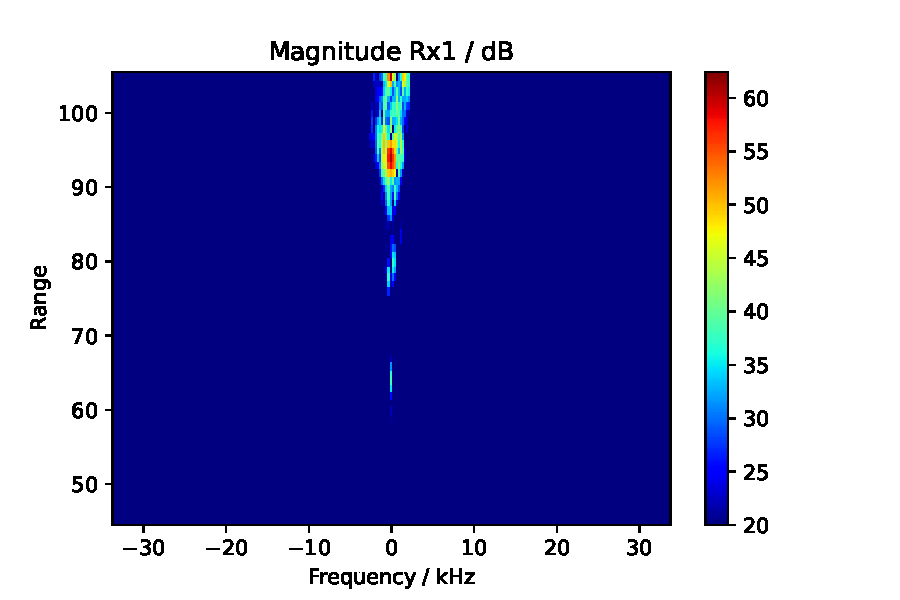
\includegraphics[width=\textwidth]{graphics/t1/t1-mag-rx1.pdf}
    \caption{Task 1: Magnitude of Spectrum of Receiver 1.}
    \label{fig:t1-mag-rx1}
    \end{minipage}\hfill
    \begin{minipage}{0.48\textwidth}
        \centering
        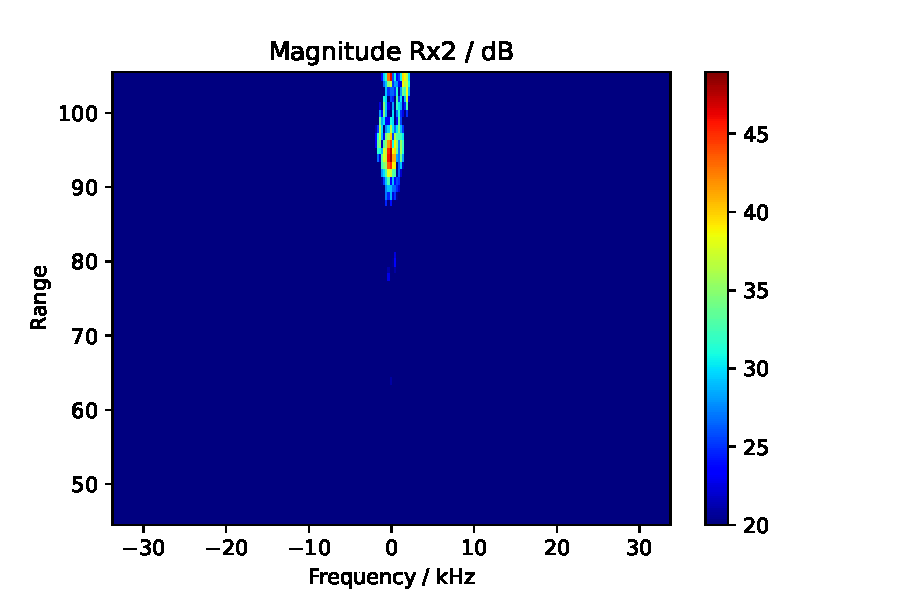
\includegraphics[width=\textwidth]{graphics/t1/t1-mag-rx2.pdf}
    \caption{Task 1: Magnitude of Spectrum of Receiver 2.}
    \label{fig:t1-mag-rx2}
    \end{minipage}
\end{figure}

\begin{figure}
    \centering
    \begin{minipage}{0.48\textwidth}
        \centering
        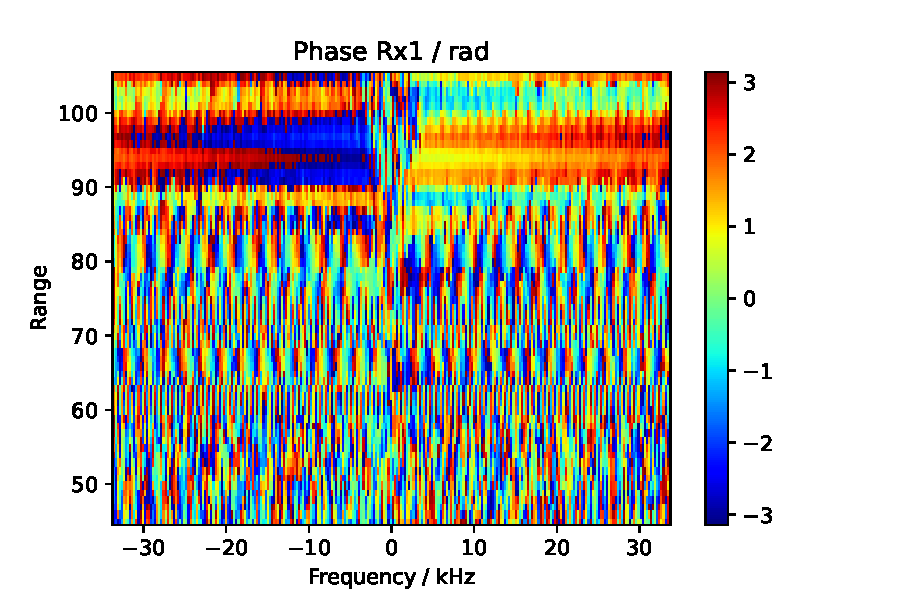
\includegraphics[width=\textwidth]{graphics/t1/t1-phase-rx1.pdf}
    \caption{Task 1: Phase of Spectrum of Receiver 1.}
    \label{fig:t1-phase-rx1}
    \end{minipage}\hfill
    \begin{minipage}{0.48\textwidth}
        \centering
        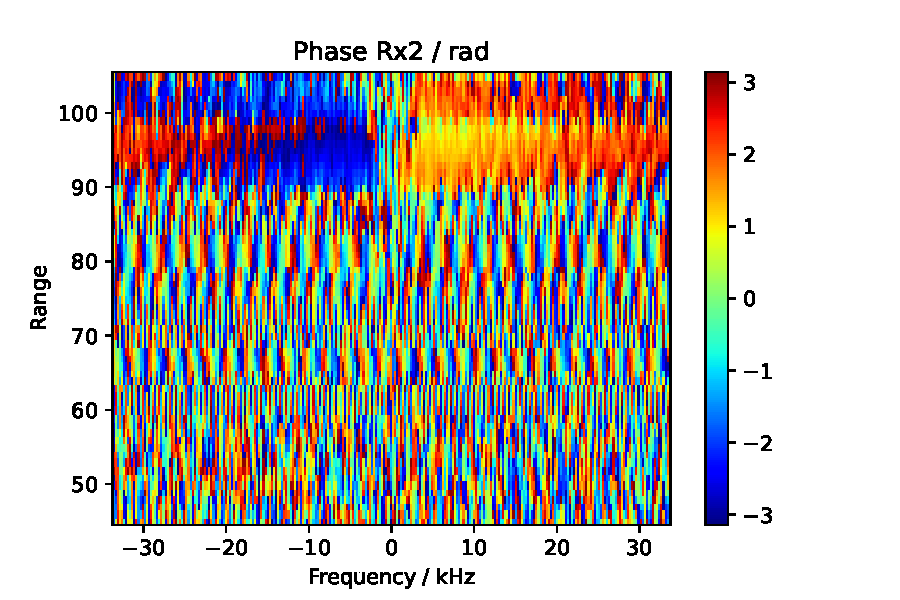
\includegraphics[width=\textwidth]{graphics/t1/t1-phase-rx2.pdf}
    \caption{Task 1: Phase of Spectrum of Receiver 2.}
    \label{fig:t1-phase-rx2}
    \end{minipage}
\end{figure}
